\chapter{Introduction}
% Goal : 5-10 page talk before the talk
% maybe not 10 pages, but providing a general overview of the paper is the goal here
\section{Motivation}
\label{sec:overview}
Mobile devices, such as smartphones and smartwatches, have a key limitation---a
limited battery life which allows them to operate for finite periods before
requiring recharging.  Resource-intensive applications, such as those involving
augmented reality or deep learning inference, exacerbate the situation by
accelerating battery depletion.  Consequently, a mobile device cannot match the
sustained performance and resource capacity of stationary computers, which are
free from the requirements of mobility. Mobile devices will always lag behind
static devices in computational ability because of their size and weight
constraints \cite{satya2014}. Increased computational ability, at the same
level of hardware efficiency, demands higher energy consumption. This requires
larger batteries to preserve operating time, thereby increasing weight and
size---which are undesirable for mobile devices.
\Cref{tab:mobility-constraints} shows how mobile devices have lagged behind
servers in computational power over a period of 25 years. This limitation has
been referred to as the ``mobile penalty'', the cost for reduction in
performance required to adhere to mobility constraints
\cite{satya-edge-native}.

\begin{table}[htbp]
    \centering
    \begin{tabular}{@{}lllll}
        \toprule & \multicolumn{2}{c}{\textbf{Typical Server}} & \multicolumn{2}{c}{\textbf{Typical Mobile Device}}\\\midrule
        \textbf{Year} & \textbf{Processor} & \textbf{Speed} & \textbf{Device} & \textbf{Speed}\\\midrule
        1997 & Intel Pentium II & 266 MHz & Palm Pilot & 16 MHz\\
        2002 & Intel Itanium & 1 GHz & Blackberry 5810 & 133 MHz\\
        2007 & Intel Core 2 Quad Q6600 & 2.4 GHz x 4 & Apple iPhone & 412 MHz\\
        2012 & Intel Xeon E5-2690 & 3.8 GHz x 8 & Samsung Galaxy S3 & 1.4 GHz x 4\\
        2017 & Intel Xeon Platinum 8180 & 3.8 GHz x 28 & Google Pixel 2 & 2.35 GHz x 4,\\
             &&&& 1.9 GHz x 4\\
        2022 & AMD EPYC 9654 & 3.7 GHz x 96 & Samsung Galaxy S22 Ultra & 3 GHz x 1,\\
             &&&& 2.5 GHz x 3,\\
             &&&& 1.8 Ghz x 4\\
        \bottomrule
    \end{tabular}
    \caption{The Mobility Penalty Over a Period of 25 Years (Adapted from Chen \cite{zchenthesis}, Flinn \cite{flinn2012cyber})}
    \label{tab:mobility-constraints}
\end{table}

This limitation is particularly problematic for unmanned aerial vehicles
(UAVs), or drones, which spend most of their energy on flight. Larger batteries
required to sustain intensive on-drone computation increases drone weight.
Increased drone weight leads to an upwards spiral in weight as larger rotors
and more powerful motors are needed to achieve the same amount of lift.  This
requires even larger batteries which, in turn, may require a more reinforced
aircraft structure, and so on. How, then, can we enable mobile devices to do
more given the mobility constraints they are subject to? Advancements in
hardware efficiency provide one possible way forward, but these advancements
are slow and far between. It turns out that there is a way to "cheat" that
enables mobile devices to do more today.

A significant body of work in the field of mobile computing has aimed to
address the inherent resource poverty of mobile devices using cloud or cloudlet
offload \cite{satya1996,satya2009}.  Cloudlet offload addresses these issues by
allowing mobile devices to remotely execute computationally expensive tasks on
cloudlets that do not need to be light or small. This allows mobile devices to
retain their low weight and small size, but possess superior computational
abilities.

SteelEagle, an autonomous drone system, follows this approach \cite{bala2024}.
Its main tenet is the use of commerical-off-the-shelf (COTS) drones, which are
readily available at low cost but typically have minimal to no on-board
computational resoures.  Utilizing cloudlet offload, SteelEagle enables COTS
drones to perform much more intelligent tasks than what they were designed for,
and exhibit autonomous capabilities typically only found in larger, more
expensive drones.  SteelEagle focuses on active vision tasks which require the
ability to perform live video analytics during flight to determine the next
course of action. SteelEagle drones relay their camera video stream over a
commercial cellular network to a nearby on-ground edge server, a cloudlet,
which runs a computationally expensive pipeline involving neural networks to
perform tasks such as object detection (\cref{fig:steeleagle-drone-arch}).  This processing of the raw drone
sensor streams allows obtaining higher level semantic information about the
drone's physical environment, such as the distance to obstacles that present
the danger of a collision. The drone can then be sent piloting commands to
react, such as instructions to actuate to avoid an impending collision.

\begin{figure}[htbp]
\centerline{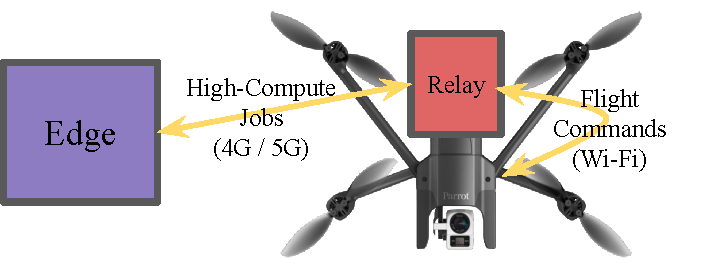
\includegraphics[width = .6\textwidth]{figs/steeleagle-drone-arch-cropped.pdf}}
\caption{Cloudlet Offload in SteelEagle}
\label{fig:steeleagle-drone-arch}
\end{figure}

An important consideration for SteelEagle is the agility of the resulting
system.  How quickly can a drone respond to a change in its environment? It is
the end-to-end latency of the entire execution pipeline, including sensing,
offloading, inferencing, decision making, and actuation, that defines the
agility. A high end-to-end latency can severely handicap the drone---it must
fly at a higher altitude or at lower speeds to be safe if it takes a long time
to identify obstacles and actuate to bypass them. Drone flight at a higher
altitude precludes close observation, and lower speeds make missions take
longer, limiting the capabilities of the drone. Search and rescue missions in
forests, and missions to aid law enforcement operations in dense cities, for
instance, must fly at low altitudes while bypassing obstacles in the
environment that present a collision risk---trees branches, streetlight poles,
utility wires, and buildings---without impacting mission speed. Unless we can
achieve high agility, SteelEagle drones will struggle to perform these missions
well.  Since these missions are one of the most compelling use cases for
autonomous drones, benchmarking the end-to-end pipeline to determine latency
bottlenecks and identifying opportunities for latency optimization is a very
worthy pursuit.

SteelEagle drones currently act as thin clients, performing no on-board
computation---they are controlled exclusively over the network. They transmit a
video stream from their camera to a cloudlet which determines the next course
of action based on an analysis of the received video, sent back to the drone
over the network. While this strategy allows treating consumer-grade
non-programmable drones as black boxes, it presents severe limitations. First,
SteelEagle drones struggle in areas with unreliable cell service and are
completely inoperable in regions without cellular coverage. Second, cloudlet
offload imposes an upper bound on drone agility as it adds the cost of a
round-trip latency to a cloudlet. As originally envisioned, cloudlets are
differentiated from clouds because of their physical proximity, which allows
application end-to-end response time to be just a few milliseconds. However, in
practice, the usage of commerical cellular networks for offload to the cloudlet
increases this latency to tens of milliseconds. This limits the agility of the
drone, as the reaction time is at least the round-trip time to the cloudlet.

This thesis explores the use of onboard computation to mitigate these issues,
and the resulting impact on drone agility. In recent years, domain-specific
system-on-a-chip devices have become available that provide substantial
energy-efficient on-board computational resources through the inclusion of
hardware accelerators in the chip design. These chips can decode the video
stream generated by the drone and perform analytics using TensorFlow Lite
models, and often include 5G and Wi-Fi connectivity. Using such a chip as a
communications relay in SteelEagle allows us to continue treating the drone as
a black box, but employ new cloudlet offload tactics that result in tighter
OODA loops for use cases that can utilize the hardware accelerators, while
retaining the generality offered by cloudlet offload.



\section{Overview}


\section{Contributions}

The contributions of this thesis include
\begin{itemize}
  \item Things
\end{itemize}


\section{Organization}
\begin{comment}
The "Observe, Orient, Decide, Act" (OODA) loop framework devised by military
strategist John R. Boyd provides a framework to structure our investigation
into the end-to-end latency of SteelEagle. According to Boyd, decision-making
happens in a continuous iteration of these steps. Boyd attributed the faster
OODA loop of U.S. pilots flyng F-86s, because of the bubble-shaped canopy
offering better visibility and hydraulic controls that allowed for easier
switching between manoeuvres, as the reason the slower F-86s fared better than
the North Korean MiG-15s during the Korean War \cite{morton1995}. A system with
a tighter OODA loop corresponds to a more agile drone. Instead of measuring
just the overall system latency, performing a break down of the latency across
the OODA steps provides more insight into system latency bottlenecks.
\end{comment}
